\chapter{BACKGROUND}
This chapter is divided into six sections.  Section \ref{bg:som} introduces
the SOM and some of its basic properties.  Next, section \ref{bg:train}
discusses the training process which allows the SOM to represent our input
data.  In section \ref{bg:topo} we explore the importance of topology in the
SOM.  The following two sections, \ref{bg:edge} and \ref{bg:sphere}, expand on
this discussion by introducing some potential problems and possible solutions
found with the traditional topologies used in SOM. Specifically, section
\ref{bg:edge} describes edge effects and section \ref{bg:sphere} describes the
use of spherical topologies which attempt to overcome these edge effects.
Finally, section \ref{bg:size} highlights the importance of the network size
in SOM.



%The first provides a general
%introduction to the SOM algorithm and the problems created by using irregular
%topology. The second reviews the current spherical topologies used with SOMs.
%The third examines the flexibility of the various topologies with regard to
%network size. The fourth takes a look at the limitations of using ``uniformity''
%to evaluate potential topologies.


%Kohonen suggests that a fundamental hierarchy can be found the ``structured occupation and utilization of a uniform memory territory'' \cite[p. 102]{Kohonen2000}.
%Artificial neural networks are a broad class of mathematical or computational models that are conceptually based on biological neural networks.
%The SOM is often classifed as a data reduction technique as it projects a high-dimensional input space onto a low-dimensional lattice, or map, of neurons.
%Kohonen mimics the ``structured occupation and utilization of a uniform memory territory'' that is found in these networks.
%He suggests that the geometric or spatial organization of information in these territories, or spaces, provides for a fundamental hierarchy.
%By creating and implanting a conceptual framework of these spaces and the process which organizes information within them,
% Kohonen is able to represent the similarities of high-dimension information as spatial 
%among input signals as relationships among samples from an input-space as 
%and the process which organizes information within this territory \cite[p. 102]{Kohonen2000}.
%In the SOM an input-space is organized onto a set of neurons through an unsupervised competitive learning process.
%The learning, or training, process organizes information onto this space by presenting input signals to the network.
%Neurons compete for input signals and winning neurons are updated to better model these signals.
%The neurons compete for the input signals and winning neurons updated in order to model them.
%The SOM follows from a conceptual understanding of the process which organizes information within this territory.  
%The neurons act as the uniform memory territory, which is structured by a network topology that defines the connections between these neurons.
%The rectangular and hexagonal topologies shown in Figure \ref{topos} are traditionally used for this purpose.
%As the learning progresses similar input signals are attracted to similar areas of the network.
\section{Self-Organizing Maps}
\label{bg:som}
The SOM is a type of artificial neural network developed by Teuvo Kohonen.  In
the SOM an input-space is organized onto a set of neurons through an
unsupervised competitive learning process \citep{Kohonen2000}. The neurons, arranged on a lattice,
compete for input signals.  The input signals are samples from an input-space.
During training the winning neurons and those around them are updated to
better model these signals. In each step of the training process the winning
neuron is the one most similar to a given input signal.  Traditionally, the
neural lattice, or network, has either a rectangular or hexagonal topology.  As shown in
Figure \ref{topos} these topologies have different properties.  In the
rectangular topology, Figure \ref{topo:rook}, neurons are bounded by four
neighbors.  In the hexagonal topology, Figure \ref{topo:hex}, neurons are
bounded by six neighbors.  In both topologies, neurons on the edge have fewer
neighbors.  As the learning progresses, \emph{data similarities} in the
high-dimensional input-space are translated into \emph{spatial relationships}
in the low-dimensional neural network \citep{ritter99}.
%As the learning progresses similar input signals become attracted to similar areas of the network, fulfilling the translation from \emph{data similarities} into \emph{spatial relationships}.

\begin{figure}
\centering
\subfigure[Rectangular Topology]{
  \label{topo:rook}
  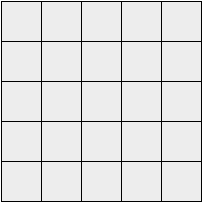
\includegraphics[width=.25\linewidth]{topo_rook.png}
}
\subfigure[Hexagonal Topology]{
  \label{topo:hex}
  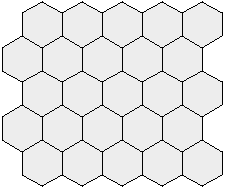
\includegraphics[width=.30\linewidth]{topo_hex.png}
}
\caption{In traditional SOM either a rectangular or hexagonal topology is used.}
\label{topos}
\end{figure}

The SOM has a number of applications, but is primarily used for data reduction
and data visualization.  The SOM is often compared with other data reduction
techniques, such as principle components or multi-dimensional scaling. Like
SOM, these techniques reduce the dimensionality of the input-space
\citep{Kohonen2000,skupin08}. However unlike SOM, these techniques do not
directly preform clustering.  The SOM on the other hand has the ability to do
both simultaneously.  That is the SOM can collapse a high dimensional
input-space into two dimensions, \emph{and} collapse observations from the
input-space into groups or clusters.  The degree to which clustering occurs is
controlled by the size of the SOM.  In smaller SOMs, as the neurons try to
model the input-space, observations are ``collected'' by the neuron which
models it most accurately.  In larger SOMs, perhaps even where there are more
neurons than observations, observations are still collected by their best
model.  However, other neurons map the intermediate areas between
observations, providing a low-dimensional spatial layout of otherwise
high-dimensional data.

\cite{skupin08} demonstrate these properties when they use state level data
from the U.S. Census Bureau to train two SOMs of different sizes.  In the
three-by-three (9) case the neurons act as containers clustering similar
states, while in the twenty-by-twenty (400) case relationships are expressed
with much finer granularity.  In the second case the SOM proves to be a very
useful visualization tool.  The similarities and dissimilarities among the
states are represented as spatial orientations and distances.  Even in this
larger case, where neurons outnumber observations, clustering may still occur.
This happens because the SOM tries to represent the entire input-space.  If
some observations are sufficiently different, while others are sufficiently
similar; the network may be better utilized by allowing some neurons to
represent dissimilarities, while clustering of observations occurs at other
neurons.

A useful property of the SOM is that the network structure between the neurons
allows us to create meaningful visualisations.  Observations used in the
training, as well as new observations from the input space, can be mapped
onto the trained surface in order to show higher dimensional relationships in a
familiar map-like form. The SOM's component planes capture the spatial layout
of each dimension, these are often visualized in a series of maps.  These
maps can provided useful information about the relationships between the
different attributes of your input-space.  In terms of information
visualization, the spatial layout of observations on the network provides far
more information than traditional methods, such as ordered lists or scatter
plots.

\section{Training}
\label{bg:train}
% the number of neurons
%and their spatial arrangement are determined before training the SOM.
%An observation from the input space is represented as input vector, \(x\).
%We must also define a distance measure \(d(x,m_i)\) between \(x\) and \(m_i\).
%For this thesis, euclidean distances are used for this purpose.
As with other artificial neural networks, the SOM has to be trained with
samples from the input-space.  These samples, or observations, are represented
as input vectors.  During the training process neurons compete for inputs;
with each training step winning neurons are adjusted to better match the
signals they receive.  Feedback between the neurons allows the entire network to
eventually coverage to a final state. After training, each neuron in the SOM
will represent a portion of the input space.  To accomplish this
representation each neuron is associated with a parametric reference vector,
\(m_i\), referred to as a model vector \citep{Kohonen2000}.  The length of the
model vectors are equal to the length of the input vectors, such that each
element within a model vector represents a dimension of the input-space.  The
initial values of the elements are most commonly randomized, such that a
mapping of the input-space onto the initial SOM would have no meaning. Other
initializations are possible and may reduce the time required for the map to
coverage \citep{Kohonen2000}.

Our implementation follows the ``Original Incremental SOM Algorithm'' as laid
out by \cite{Kohonen2000}.  In each step of the algorithm, a randomly select
observation (input vector $x$) searches for its best model (reference vector
$m_i$) among the neurons.  The best model is defined as the $m_i$ with the
smallest distance to $x$.  These distances are referred to as quantization
errors (QErrors), and they measure the distance between two vectors in
attribute space \citep{Kohonen2000}.  Our implementation uses Euclidean
distances, however, any reasonable distance measure can be used here.  The
``winning'' neuron is termed the Best Matching Unit (BMU $c$).  The
neighborhood ($N_c$) around the BMU ($c$) is found and all $m_i$ within $N_c$ are
updated.  The size of the neighborhood and the magnitude of the updates are
controlled by the neighborhood function. In our implementation, the width of
the neighborhood decreases as the training progresses, and the magnitude of
the updates decrease, with a Gaussian function, toward the edge of the
neighborhood. A learning-rate factor is used to further reduce the magnitude
of the updates as training progresses.  Combined these create the neighborhood
kernel function $h_{ci}$ which defines a scaler used to adjust the magnitude
of each update in a given training step.  This function always evaluates to
zero for neurons outside the neighborhood.  The update is defined as,
\begin{equation}
  {m_i(t+1)} = m_i(t) +  h_{ci}(t)[x(t) - m_i(t)]
\label{update}
\end{equation}
where, $t$ is the current training step.  The training process is repeated a
predefined number of times, or ideally until the map converges.

\section{Topology}
\label{bg:topo}
\citeauthor{wu2006} state that ``[f]or SOM, it is desirable to have all
neurons receive equal geometrical treatment'' \cite[p. 900]{wu2006}.  To
satisfy this constraint, two conditions must be met.  First, each neuron
should occupy the same amount of space on the given surface.  Second, each
neuron should be bordered by the same number of surrounding neurons, and we
should maximize that number.  The first condition is largely irrelevant in the
training of the SOM.  However, visualizations that do not have uniformly sized
and spaced neurons could potentially mislead an untrained viewer, as larger
neurons may appear to be more significant. Of greater importance to
training is the SOM's topology, as it describes how the neurons are connected
within the network.  In training the topology defines, $N_c$, the neighborhood
around the winning neurons, and irregular topologies directly impact the size and
shape of these neighborhoods.  
%According to \cite{wu2006}, the hexagonal structure is more uniform and generally preferred.

We believe the regularity of a given topology is a better metric
for evaluating different topologies for use in SOM. In graph theory a regular
graph, is simply a graph in which every node has the same number of neighbors
\citep{harris2000}. A measure of regularity tells us how uniform neurons
are in terms of their connections to other neurons in the network. In network
theory, nodes with more connections are thought to be more central to the network and have a
larger influence than nodes with fewer connections \citep{Wasserman:1994}. A simple measure for
capturing this is degree centrality.  The degree (number
of adjacent neurons) is measured for each neuron in the network. The variance
in these measurements tells how regular the network is, a perfectly regular
topology should have a variance equal to zero.  Other methods, such as closeness
centrality compare nodes based on their connectedness to every node in the
network.

\section{The Boundary Effect}
\label{bg:edge}
Traditionally the SOM is laid out on a two-dimensional plane using either a
rectangular or hexagonal topology.  Both of these topologies are irregular,
because neurons on the boundary of the network have fewer neighbors.  Neurons
with fewer neighbors have fewer chances of being
updated \citep{wu2006}.  As observed in Figure \ref{som:states}, neurons in
the center of the map tend to better represent the mean of the input-space.
In this SOM we used the same data as \cite{skupin08} to map the fifty states
and the District of Columbia onto a SOM trained with thirty-two population
census variables. After training, we measured the distance between each
neuron's model vector, $m_i$, and the mean of the input vectors, $\bar{x}$.
Darker neurons have a relatively larger difference from the mean of the input-space,
while lighter neurons are relatively closer. We also measured the difference
of each observation to the mean $\bar{x}$, these distances are represented by
the size of the point symbols.  Larger symbols are farther from the mean. The
five observations furthest from the mean: Alaska, District of Columbia,
Hawaii, Maine, and Utah are highlighted with bold labels.  The five
observations closest to the mean: Alabama, Illinois, Louisiana, Nebraska and
North Carolina have underlined labels.  Arguably the outliers are being pushed
to the edges of the map, where they encounter fewer competing signals.
Edge effects are also common in spatial analysis, for example in point
patterns the edge of a study unit may hide the true distribution of an
observed pattern.  In SOM the edge of the neural lattice represents a true
boundary, which effects its ability to represent \emph{data similarities} as
\emph{spatial relationships}.

\begin{figure}[htb]
\centering
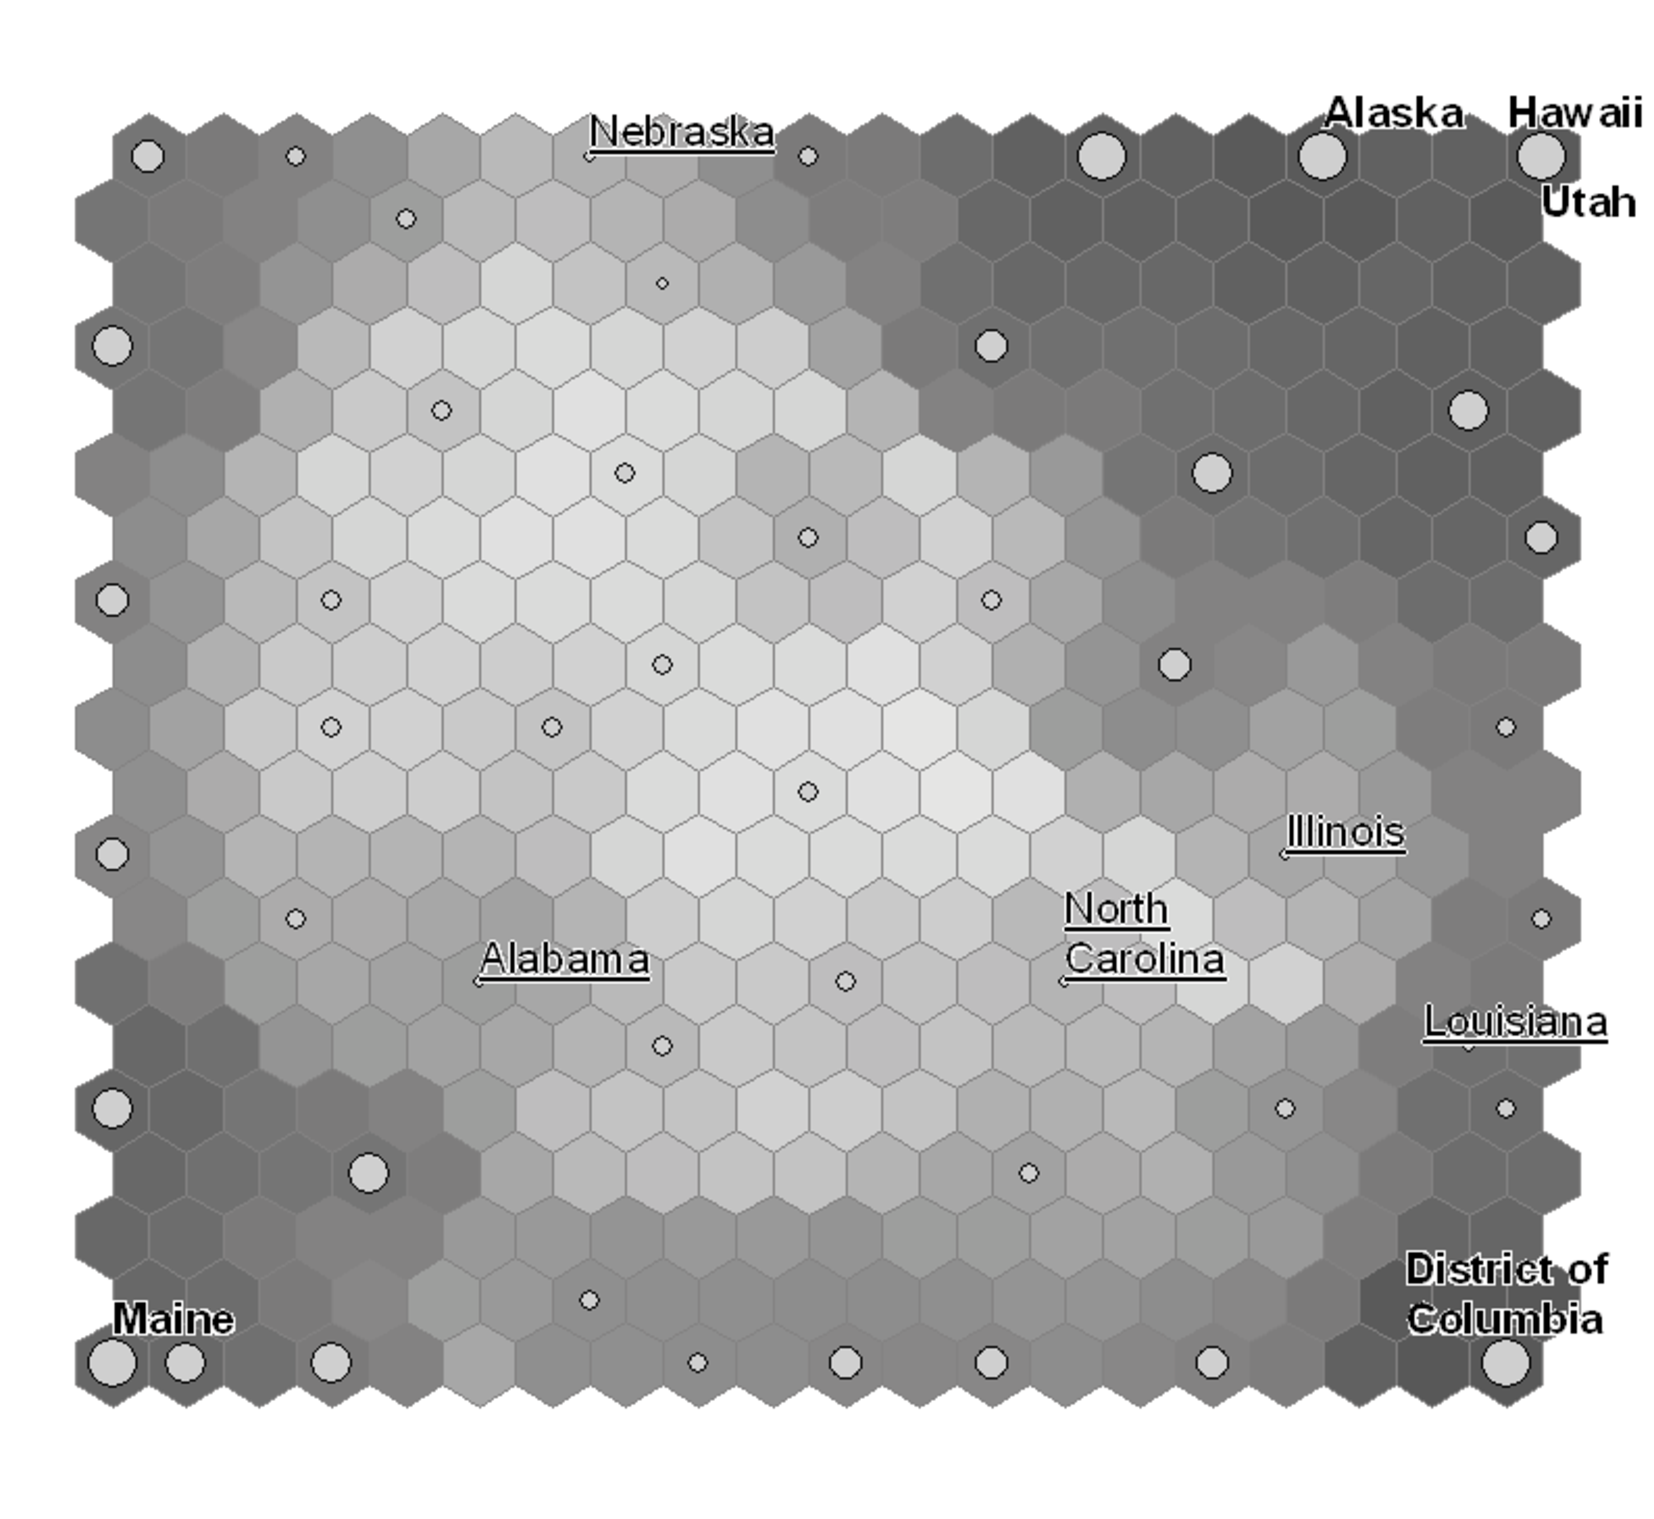
\includegraphics[width=.9\linewidth]{gridedge_grey.pdf}
\caption{An example of the boundary effect in SOM.}
\label{som:states}
\end{figure}

One way to eliminate the edge effect is to wrap the lattice around a
three-dimensional object such as a sphere or torus, thereby removing the edge
entirely. The toroidal SOM was introduced by \cite{li1993}, however the torus
is not effective for visualization, as maps generated from a torus are not
very intuitive \citep{ito2000,wu2006}.  \cite{ritter99} describes the torus as
being topologically flat and suggests that a curved topology, such as that of
a sphere, may better reflect directional data.  A sphere also results in a
more intuitive map, since we are accustomed to looking at geographic maps
based on a sphere.  

\section{Spherical SOM}
\label{bg:sphere}
\cite{ritter99} first introduced the spherical SOM, and several enhancements have
since been suggested \citep{boudjemai2003,sangole03,Nishio:2006fk,wu2006}.  A
good comparison of these enhancements can be found in \cite{wu2006}.  All of
these methods derive their spherical structure through the tessellation of a
polyhedron as originally proposed by \cite{ritter99}.  \cite{wu2006} point
out the importance of a uniform distribution on the sphere, and that it is
preferable for all neurons to have an equal number of neighbors and to be
equally spaced.  They find generally that the tessellation method best satisfies
these conditions, and specifically that the icosahedron is the best starting
point \citep{wu2005}. Tessellation of the icosahedron results in a network of
neurons, each having exactly six neighbors, save the original twelve
which each have five neighbors.  This is very close to the ideal structure in
which every neuron would have exactly six neighbors.  \cite{wu2006} prefer
these this structure, because it has very low variances in both neuron spacing
and neighborhood size. 

Based solely on measures of neuron spacing, \cite{wu2005} dismissed the usefulness of a method
proposed by \cite{Rakhmanov94} for distributing points on a sphere.  Similarly
\cite{Nishio:2006fk} use these variance measures to support their helix
algorithm for distributing points on a sphere.  Table \ref{table1} shows that
these metrics can be misleading and comparison across topologies may not be
consistent.  The traditional rectangular and hexagonal topologies have no
variance in neuron spacing, and the generally preferred hexagonal structure
displays greater variance in neighborhood size than the rectangular structure.
The torus, by comparison, would have variance in neuron spacing, yet no
variance in neighborhood size.  The distance between two neurons is only
considered during the formation of the neural network.  At this stage the
spacing is significant as it plays a part in constructing the network's
topology by determining neuron adjacency.  However, using this measure to
evaluate potential topologies for use in SOM may be misleading.

\begin{table}[htbp]
\caption{Variances in Topologies}
\begin{center}
\begin{tabular}{|c|c|c|c|}
\hline
Topology&Grid Size&Neuron Spacing&Variance in Neighborhood Size\\
\hline
Rectangular&9x18&1&0.2716\\
Hexagonal&9x18&1&1.2138\\
Tessellation&162&0.25319 - 0.31287& 0.0686\\
Rakhmanov&162&0.15779 - 0.30069& 0.2908\\
\hline
\end{tabular}
\end{center}
\label{table1}
\end{table}

As spherical (and other alternative) topologies become
increasingly more common it is necessary to investigate how the choice of
topology effects the SOM.  In this thesis the effect of irregularity within
topologies is studied as an attempt to investigate not only the edge effect,
but also to help facilitate the comparison of topologies.  It is important to
note that spherical topologies may not be appropriate for all applications.
Removing the edge may reduce the SOM's ability to converge.  As outliers are
forced to interact they introduce more competition among the neurons.  We
would also expect outliers to occupy more space in the final map as their
dissimilarity in attribute space should translate to more distant spatial
relationships in the trained SOM.  More research will be needed to help researches
determine the most appropriate topology for their data and research objectives.

\section{Network Size}
\label{bg:size}
The number of neurons used in the SOM is a decision the research must make and
is both a function of the size of their dataset and the purpose for which the
SOM is to be used.  Generally speaking fewer neurons would be used in a
clustering application while larger SOMs are commonly used for visualizing
high-dimensional datasets.  The literature offers little theoretical guidance
on choosing an appropriate network size for a given dataset \citep{cho1996}.
\cite{toolbox} suggests that the network size should be ``as big as
possible,'' but also states that this becomes computational impractical for
larger problems. As a general rule-of-thumb, \citeauthor{toolbox} suggests using a
network size of \(5\sqrt {n}\), where \(n\) is the number of observations. The
application for which this network size would be most relevant is unclear.  

\begin{figure}[htb]
\centering
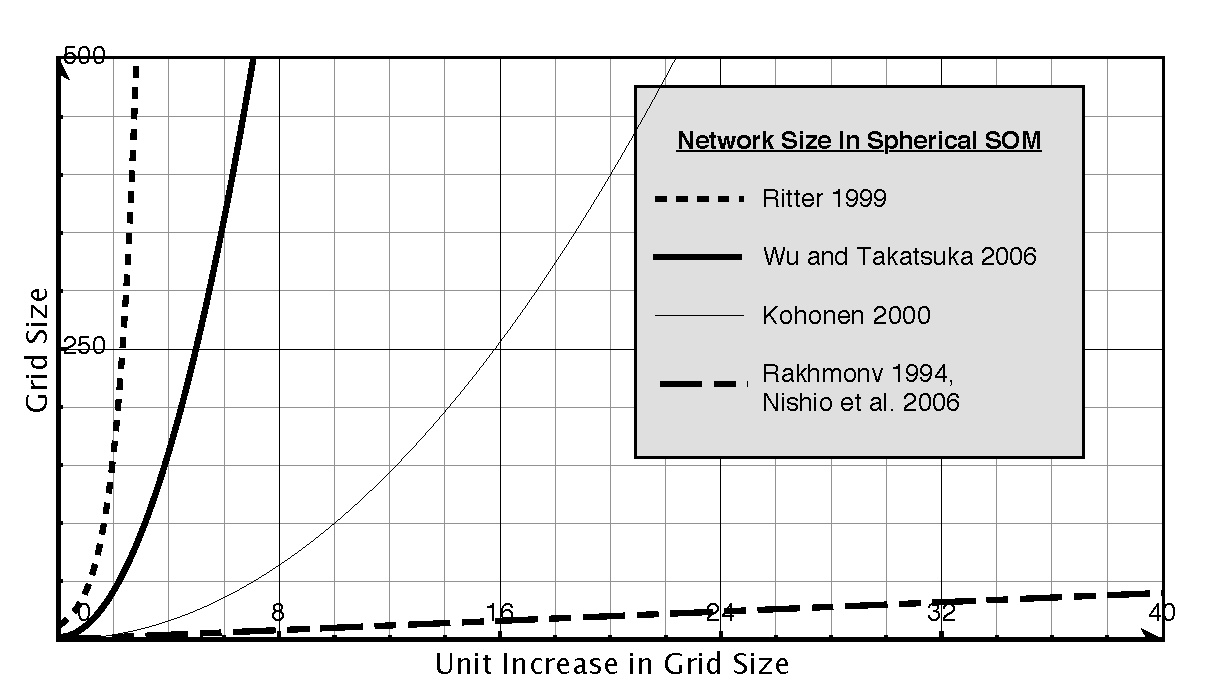
\includegraphics[width=\linewidth]{networkSize.pdf}
\caption{This figure demonstrates the achievable network size using various
spherical topologies, in comparison with the traditional SOM. The Y-axis
represents the achievable network size, while the X-axis represents the
smallest increase in grid size for each topology.}
% frequency of the tessellation. For the traditional Kohonen method the X-axis represents the size of both dimensions of the grid; for comparability the ratio between the dimensions was fixed at one ($X_{dim}=Y_{dim}$).  For the \cite{Rakhmanov94} and \cite{Nishio:2006fk} methods the X-axis represents the exact network size.}
\label{fig:nSize}
\end{figure}

Given this lack of theoretical development, researchers should be cautious
when using methods that limit the control of network size.  Having a high
level of control over network size allows support for such very different SOM
applications as clustering versus low-dimensional spatial layout.
Figure \ref{fig:nSize} shows how the achievable network size varies between
topologies.  In rectangular and hexagonal SOMs it is undesirable to have one dimension
drastically larger than another, as such there are practical limitations to
the size of these networks.  As an aside, the preferred ratio between these
dimensions depends on the data being represented, and should generally not
equal one \citep{kohonen1996, toolbox}.  In Figure \ref{fig:nSize} we used a
ratio of one only for comparison purposes with the other topologies.
\citeauthor{ritter99}'s tessellation method results in a network size that
grows at a rate of \(N=2+10*4^f\), where $f$ is the frequency of tessellation.
\cite{wu2006} offer a slight improvement. Rather than recursively subdividing
the faces, they redivide the original icosahedron with each step, resulting in
\(N=2+10*f^2\).  Methods for arranging an arbitrary number of points on a
sphere provide the highest degree of flexibility when choosing a network
size.  For example, the method proposed by \cite{Rakhmanov94} can
distribute any number of points onto the surface of a sphere.  Strictly
speaking, this is not a topology in itself, as no connections are defined
between the points. In our implementation we create a spherical topology be
applying Delaunay triangulation to these points \citep{Ranka97}.  We refer to
this topology simply as ``spherical''. Using \citeauthor{ritter99}'s method
with a tessellation frequency of three, would result in 642 neurons, the next
smallest size is 162 neurons.  The geodesic topology offers three additional
levels between 162 and 642 neurons (252, 362, 492).  Using the spherical
topology however, we are not limited to these network sizes.

Similarly \cite{Nishio:2006fk} try to address the issue of network size
granularity by departing from the tessellation method and suggesting the use
of a partitioned helix to uniformly distribute any number of neurons on a
sphere.  The method proposed by \cite{Rakhmanov94} was dismissed by
\cite{wu2005} for failing to satisfy the uniformity conditions described
above. \cite{Nishio:2006fk} suggest their method for distributing points
satisfies these uniformity constraints, however they do not describe a network
topology.  It is unclear how they define neighbor relationships and without
clarification we cannot implement their topology.  Methods for distributing
points on the sphere, which allow for fine-grained control over network size,
produce slightly more irregular topologies.  However, no substantive
discussion of these irregularities or their effects on SOM training exists in
the literature. Network size plays an import role in the SOM and given
that limited theoretical guidance is available for choosing network size,
researches should be cautious when using topologies that limit control over
this parameter.  Particularly for larger SOMs, the desired network size may
not be achievable via tessellation of the icosahedron.

